\documentclass[a4paper, 10pt, final, garamond]{book}
\usepackage{cours-preambule}

\titleformat{\item}{}{\arabic{item})}{.5em}{}{}
\titleformat{\subitem}{}{\arabic{item}) \alph{subitem} --}{.5em}
{}{}

\makeatletter
\renewcommand{\@chapapp}{Devoir surveill\'e -- num\'ero}
\makeatother

\begin{document}
\setcounter{chapter}{4}

\chapter{Commentaires sur le DS n\degree5}

\begin{NCprop}[width=\linewidth]{\centering\bfseries\ Rappel des malus}
    Chacune des lettres suivantes sur vos copies sont des malus de \num{1}
    point.\smallbreak
    \begin{minipage}{0.50\linewidth}
        \begin{itemize}
            \item A~: application numérique mal faite~;
            \item V~: confusion ou oubli de vecteurs~;
            \item P~: prénom sur copies manquant~;
            \item M~: marge non laissée ou trop grande~;
            \item Q~: numéro de question mal indiqué~;
        \end{itemize}
    \end{minipage}
    \begin{minipage}{0.50\linewidth}
        \begin{itemize}
            \item E~: absence criant d'encadrement~;
            \item U~: unité manquante ou mauvaise~;
            \item H~: homogénéité non respectée~;
            \item S~: chiffres significatifs non respectés~;
            \item $\f$~: loi physique fondamentale brisée.
        \end{itemize}
    \end{minipage}
\end{NCprop}

\section{Commentaires généraux}

DS à 34 personnes, assez bien réussi~: le nombre de points le plus bas remonte,
et la moyenne pour ce DS est à 11/20. Vous avez globalement bien progressé
depuis le début de l'année, les applications numériques sont beaucoup plus
propres, les expressions littérales sont le plus souvent détaillées complètement
avant l'application numérique. Bravo~! \bigbreak

DS assez particulier, beaucoup de points à prendre principalement sur les
premières question de chaque exercice~; rares sont les personnes ayant essayé le
problème, mais au moins la base est maîtrisée. Faites attention pour le prochain
DS avec l'approche énergétique… ça coince souvent. Entraînez-vous en proportion.
\bigbreak

Malus total cumulé~: \textbf{100}. Points de la meilleure copie~: 99. Encore un
effort, un jour la tendance sera inverse~! Malus -M cumulés comme annoncé
précédemment, jusqu'à 3 pour une copie. 3 copies sans malus, bravo~: points
bonus \textbf{«~zéro malus~»} associés~; par contre les copies avec 6 malus et
plus augmentent. \bigbreak

\begin{itemize}
    \item RéférenTiel, pas référen\cancel{c}iel (même si c'est joli)~;
    \item Littéral avant numérique~;
    \item Attention aux chiffres significatifs~;
    \item N'oubliez pas d'établir le système, ce sont des points gratuits.
    \item Donnez le repérage et notamment $\af = \zpp\uz$.
\end{itemize}

\begin{framed}
    \centering\large\bfseries
    Si on vous demande d'indiquer la réponse, indiquez la réponse~: points pour
    «~réponse A~» et assimilé.
\end{framed}

\begin{multicols}{2}
\section{Exercice 1 \hfill \textcolor{red}{/21}}
\begin{enumerate}
    \item Points pour le schéma avec projetés. Le chemin est $n\times\ABr$ 
        (souvent noté $(\ABr)$ entre parenthèses, pour différencier de $\ABr$ la
        distance simple)~: il faut justifier $n=1$. \hfill
        \textcolor{ForestGreen}{/10}
    \item Cf. TD \hfill \textcolor{ForestGreen}{/3}
    \item On ne pouvait pas calculer $x_c$, il fallait juste dire que la frange
        s'est déplacée de $x_c$. ATTENTION~: on ne peut pas négliger une valeur
        dans une expression \textit{juste} parce qu'elle est petite devant une
        autre. $3+0 = 3$, mais $3\times0 = … 0$. \hfill
        \textcolor{ForestGreen}{/4}
    \item 3 chiffres significatifs (CS). \hfill \textcolor{ForestGreen}{/2}
    \item Cf.\ corrigé. \hfill \textcolor{ForestGreen}{/2}
\end{enumerate}
\vspace*{\fill}

\columnbreak
\section{Exercice 2 \hfill \textcolor{red}{/28}}

\begin{enumerate}
    \item $v = d/t$ \textbf{si le mouvement est uniforme}. Attention, À RETIRER
        DE VOS TÊTES~: \textbf{VITESSE UNIFORME $\neq$ ACCÉLÉRATION NULLE}. Cf.\
        Frenet. \hfill \textcolor{ForestGreen}{/5}
    \item Frenet ou coordonnées polaires, mais \textbf{littéral avant
        numérique}. \hfill \textcolor{ForestGreen}{/7}
    \item RAS \hfill \textcolor{ForestGreen}{/4}
    \item Points pour un schéma. Littéral avant numérique. Plusieurs approches
        considérées comme justes. \hfill \textcolor{ForestGreen}{/6}
    \item RAS \hfill \textcolor{ForestGreen}{/3}
    \item Faites attention quand vous faites des approximations. Utilisez bien
        votre calculatrice, notamment l'astuce de mettre des valeurs dans
        des lettres pour les réutiliser que je vous ai montrée. Si on garde $t_r
        = \SI{2.7}{s}$, oui on trouve \SI{12.5}{cm}. Pas en faisant le calcul
        complet. \hfill \textcolor{ForestGreen}{/3}
\end{enumerate}
\end{multicols}

\begin{multicols}{2}
\section{Exercice 3 \hfill \textcolor{red}{/43}}
\begin{enumerate}
    \item Établissement du système important. Si exercice commencé à la partie
        2, les poins associés ont été reportés à la question 3. Point pour la
        figure. \hfill \textcolor{ForestGreen}{/10}
    \item 2 CS \hfill \textcolor{ForestGreen}{/3}
    \item À l'équilibre, $\ell = \ell_e$, $\vf = \of$ donc bilan des forces à
        faire à l'équilibre. Point pour la figure. \hfill
        \textcolor{ForestGreen}{/5 ou 10}
    \item Attention, $\ell = \ell_e + z$. Erreur classique sur les ressorts
        verticaux. Faites vos schémas. Vous ne pouvez pas mettre les constantes
        sous le tapis par changement de variable inopiné. \hfill
        \textcolor{ForestGreen}{/9}
    \item Il faut toujours savoir résoudre les oscillateurs amortis. Vous n'y
        échapperez pas~! \hfill \textcolor{ForestGreen}{/8}
    \item RAS \hfill \textcolor{ForestGreen}{/4}
    \item RAS \hfill \textcolor{ForestGreen}{/4}
\end{enumerate}
\columnbreak
\section{Exercice 4 \hfill \textcolor{red}{/24}}
\begin{enumerate}
    \item $t$ n'est pas $z$~! 2 ou 3 CS acceptés. \hfill
        \textcolor{ForestGreen}{/14}
    \item RAS \hfill \textcolor{ForestGreen}{/2}
    \item Vitesse limite $\Ra$ constante, pas besoin d'adimensionner. \hfill
        \textcolor{ForestGreen}{/2}
    \item \textbf{Littéral avec numérique}. Non seulement parce qu'il y a des
        points faits pour, mais surtout parce que ça évite le report d'erreurs
        de calculatrice… 2, 3 CS acceptés. \SI{150}{km.h^{-1}} reste surestimé.
        \hfill \textcolor{ForestGreen}{/4}
    \item RAS. \hfill \textcolor{ForestGreen}{/2}
\end{enumerate}
\end{multicols}

\begin{multicols}{2}
\section{Exercice 5 \hfill \textcolor{red}{/25}}
\begin{enumerate}
    \item Points pour $\vf = \dv{\OM}{t}$, $\dv{\er}{t} = \tp\et$, $\dv{\et}{t}
        = -\tp\er$, mais pas pour la projection sur $\ex$ et $\ey$. Soyez
        efficaces~! $k$ d'unité \si{m.s^{-1}} donc homogène à une vitesse.
        $\tpp$ ne peut pas être nul~: c'est $\ddot{\ell} = 0$.
        \hfill \textcolor{ForestGreen}{/10}
    \item Beaucoup de mélange de réponses sur cet exercice… lisez bien l'énoncé.
        Sinon projections ok. \hfill \textcolor{ForestGreen}{/3}
    \item RAS \hfill \textcolor{ForestGreen}{/5}
    \item RAS \hfill \textcolor{ForestGreen}{/2}
    \item On lit $\tp(0) = \SI{0}{rad.s^{-1}}$ sur le graphique. 2 CS ici.
        \hfill \textcolor{ForestGreen}{/3}
    \item RAS \hfill \textcolor{ForestGreen}{/2}
\end{enumerate}
\columnbreak
\section{Problème \hfill \textcolor{red}{/47}}
\begin{enumerate}
    \item Attention, $\w = \cte$. Re-points pour dérivées de $\ur$ et $\ut$.
        Point pour base sur schéma. \hfill \textcolor{ForestGreen}{/7}
    \item C'est dommage, exercice traité en soutien \SI{28}{h} plus tôt. Pas de
        frottements veut dire réaction nulle dans la direction du mouvement,
        soit $\ur$. Un point pour la représentation des forces sur schéma.
        \hfill \textcolor{ForestGreen}{/10}
    \item Cf.\ correction TD ou DS. Il faut savoir poser l'équation
        caractéristique. \hfill \textcolor{ForestGreen}{/6}
    \item RAS pour toute la suite… Q4\textcolor{ForestGreen}{/2},
        Q5\textcolor{ForestGreen}{/3}, 2CS, Q6\textcolor{ForestGreen}{/2}
        Q7\textcolor{ForestGreen}{/3} Q8\textcolor{ForestGreen}{/3} 2CS,
        Q9\textcolor{ForestGreen}{/5} on retrouve exercice 3,
        Q10a\textcolor{ForestGreen}{/4}, Q10b\textcolor{ForestGreen}{/2}
\end{enumerate}
\end{multicols}

\vfill

\begin{center}
    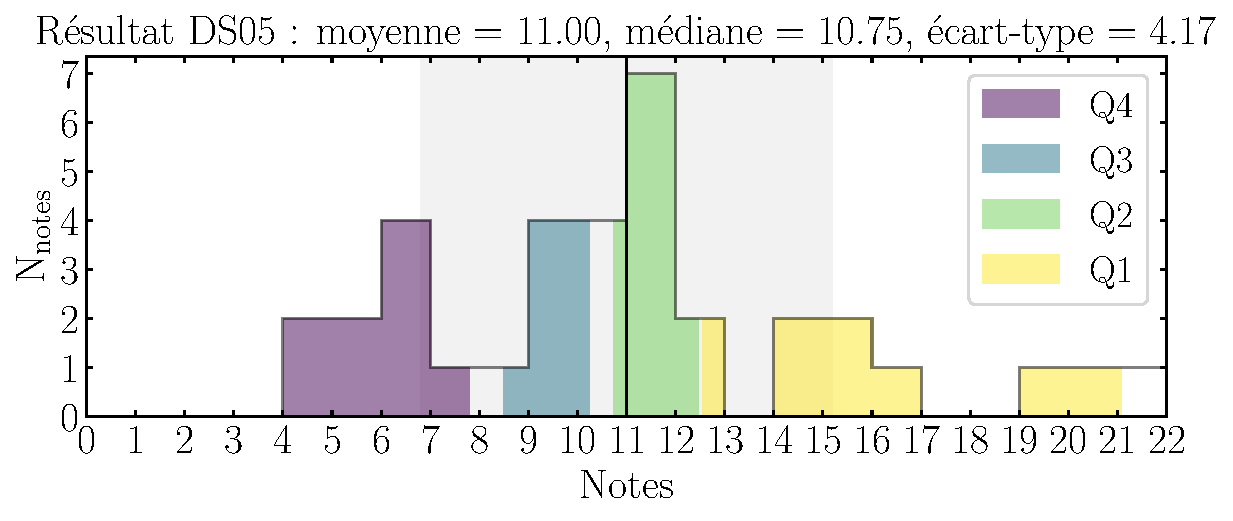
\includegraphics[width=.72\linewidth]{res_DS05.pdf}
\end{center}

\vfill

\end{document}
